\documentclass{article}
\usepackage[utf8]{inputenc}
% Margins
\topmargin=-0.45in
\evensidemargin=0in
\oddsidemargin=0in
\textwidth=6.5in
\textheight=9.0in
\headsep=0.25in

\linespread{1.1} % Line spacing

\usepackage{natbib}
\usepackage{graphicx}
\begin{document}


\title{Recuperación parcial 1}
\author{Gabriel Chavarria, 20181386, chavarria181386@unis.edu.gt}
\date{14 de Agosto del 2018}

\maketitle

\section{Pregunta #1}
\begin{enumerate}
        \item{ Conjunto de nodos: \left\lbrace 1,2,3,4,5,6,7\right\rbrace}
        
       
        
        \item{Conjunto de vértices:     \newline\left\lbrace<1,2>,<1,3>,<1,4>,<1,5>\right\rbrace 
        \newline\left\lbrace<1,6>,<4,2>,<5,2>,<5,3>\right\rbrace 
        \newline\left\lbrace<5,6>,<5,7>,<6,2>,<6,3>\right\rbrace 
        \newline\left\lbrace<7,6>,<7,4>,<7,3>,<4,3>\right\rbrace\\ 
         
        
        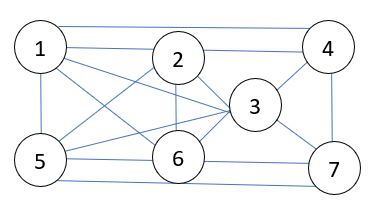
\includegraphics{1}
        }
        
         \end{enumerate}        
                


\section{Pregunta 2}
 \begin{center}
     \sum_{i=1}^{n}{n}=\frac{n(n+1)}{2}\\
\end{center}
\begin{flushleft}
Caso base n=1\\
{1}=  {1(1+1)}/{2}\\
{1}={2}/{2}\\ 
{1}=1\\
\end{flushleft} 
Caso inductivo n= n+1 \\


\begin{equation}
(1+2+3....n)+(n+1)=\frac{(n+1)(n+1)+1}{2}\\
\end{equation}

\begin{equation}
=\frac{(n+1)(n+1)+1}{2}\\
\end{equation}

\begin{equation}
=\frac{(n+1)(n+2)}{2}\\
\end{equation}

\begin{equation}
\underline{n=\frac{(n+1)(n+1)+1)}{2}}    
\end{equation}





\section{Pregunta 3}
 \sum(n)=1+2+3+4+\ \ldots\ +n\\
\[
       \sum(n)=1+2+3+4+\ \ldots\ n=
                \left\{
                        \begin{array}{ll}
                                0  & \mbox{si } n = 0 \\
                                1 & \mbox{si } n = 1 \\
                                \frac{n(n+1)}{2} & \mbox{si } n = s(i) \\
                                
                                
                        \end{array}
                \right.
\]
 


\section{Pregunta 4}

Demostrar por medio de inducci\'on la comutatividad de la suma de
numeros naturales unarios: $a\oplus b = b\oplus a$\\
Caso base a=0\\
0 \oplus b = b \oplus 0\\
\underline{b=b} \\
*($a \oplus b = b$ si $a=0$)

Caso inductivo a= s(i)\\
$s(i)\oplus b = b\oplus s(i)$\\
\underline{$s(i\oplus b) = s(i \oplus b)$}\\










\section{Pregunta 5}

Demostrar utilizando inducci\'on que $((n\oplus n)\geq n) = s(o)$.\\
Caso base n=0\\
$(0+0)\geq0= (s(0) $\\
Caso inductivo $n=s(i)$\\
s(i)\oplus s(i) \geq s(i)  \\
s(s(i) \geq s(i)  \\
s(s(i)\ominus s(i) \geq 0  \\
s(i) \geq 0  \\
\underline{s(i) \geq 0= s(0) } \\



\end{document}
